%% Problema: deve essere grassetto nella ToC e nel titolo del capitolo, ma non grassetto nell'header.
\chapter{Signal event selection}
\label{cap:event_selection}

\section{Prefiltering}
\label{sec:prefilter}
I grafici necessari probabilmente ha senso metterli qui. Magari puoi cambiare il nome in "prefiltering and data characteristics".

\begin{figure}[t]
	\centering
	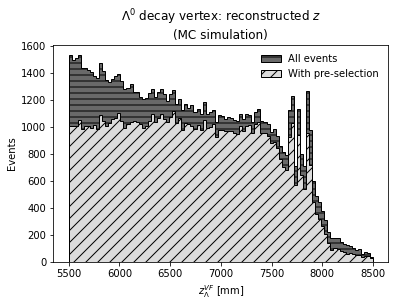
\includegraphics[width=.6\textwidth]{graphics/04-event_selection/Lambda_endvertex_z.png}
	\caption[Z.]{Distribution of reconstructed $z_\Lambda^\text{vtx}$ in simulated $\Lambda_b^0 \rightarrow J/\psi~\Lambda^0$ events, without (\textit{dark grey}) and with (\textit{light grey}) prefiltering.}
\end{figure}

\begin{figure}[t]
	\centering
	\begin{subfigure}{.45\textwidth}
		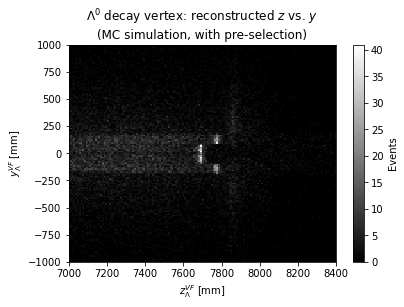
\includegraphics[width=\textwidth]{graphics/04-event_selection/Lambda_endvertex_z_vs_x.png}
		\caption{}
	\end{subfigure}
	\begin{subfigure}{.45\textwidth}
		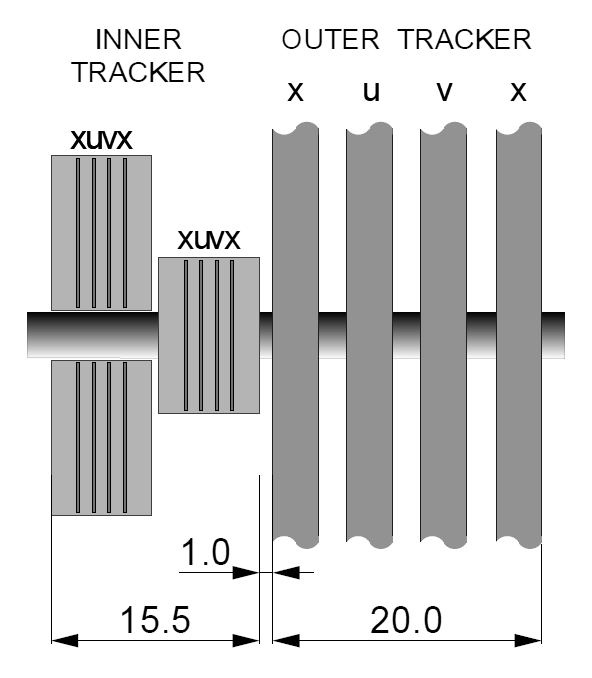
\includegraphics[width=\textwidth]{graphics/04-event_selection/t_station_top_view.png}
		\caption{}
	\end{subfigure}
	\caption[A and b.]{\textit{Left}: event distribution of simulated $\Lambda_b^0$ signal events as a function of reconstructed $x_\Lambda^\text{vtx}$ and $z_\Lambda^\text{vtx}$. \textit{Right}: top view diagram of a T tracking station (dimensions along the beam axis given in \si{\centi\meter}, lateral dimensions not to scale) \cite{Barbosa-Marinho:582793}.}
\end{figure}

\subsection{Bias in $\Lambda^0$ decay vertex}
\label{sec:lambda_endvertex_bias}
Qui devi menzionare l'orizzontalità, perché vi faccio riferimento nel Cap. 3. Devi dire che c'è il problema.

\section{HBDT classifier}
\label{sec:HBDT}

\subsection{Training data}

\subsection{Hyperparameter optimization and performance test}

\subsection{Threshold optimization}

\section{Physical background veto}
\label{sec:B0_veto}

\section{Performance on data}
Gli invariant mass fits, essenzialmente.